\usetikzlibrary{patterns}
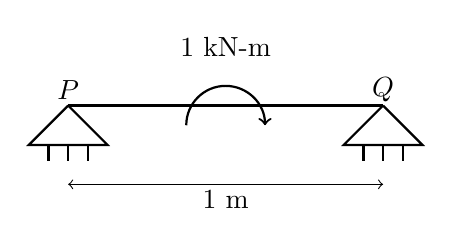
\begin{tikzpicture}
    \draw[thick] (0,0) -- (4,0);
    \draw[thick] (0,0) -- (-0.5,-0.5) -- (0.5,-0.5) -- (0,0);
    \draw[thick] (-0.3,-0.5) -- (0.3,-0.5);
    \foreach \i in {-0.25, 0, 0.25}
    \draw[thick] (\i,-0.5) -- (\i,-0.7);
    \draw[thick] (4,0) -- (3.5,-0.5) -- (4.5,-0.5) -- (4,0);
    \draw[thick] (3.7,-0.5) -- (4.3,-0.5);
    \foreach \i in {3.75, 4, 4.25}
    \draw[thick] (\i,-0.5) -- (\i,-0.7);
    \node at (0,0.2) {$P$};
    \node at (4,0.2) {$Q$};
    \draw[thick, ->] (1.5,-0.25) arc[start angle=180,end angle=0,radius=0.5];
    \node at (2,0.75) {1 kN-m};
    \draw[<->] (0,-1) -- (4,-1);
    \node at (2,-1.2) {1 m};
\end{tikzpicture}


